

%Peter W.
%Requires the memoir class (as of this date v1.6180339e 2009/02/17)
%I suggest
\documentclass[oneside,11pt]{memoir}
%%% with the wide textblock, 12pt is too small for reading ease, so best not
%%% to use 11pt or 10pt.

%%% Arial
%\usepackage[T1]{fontenc}
%\usepackage[scaled]{uarial}
%\renewcommand*\familydefault{\sfdefault} %% Only if the base font of the document is to be sans serif

%%% Garamond
%\usepackage[T1]{fontenc}
%\usepackage{lmodern}
%\usepackage{garamond}

%%% MS San Serif
%\usepackage[T1]{fontenc}
%\usepackage[scaled]{helvet}
%\renewcommand*\familydefault{\sfdefault} %% Only if the base font of the document is to be sans serif

%%% Times
\usepackage{mathptmx}  % Times New Roman, but if you have Garamond then use it;
                       % you are writing a book, not a newspaper column
\DoubleSpacing         % memoir's double spacing
\usepackage{pwasu}     % this package

%%%%%%Added by Craig Picone to meet ASU's margin requirements
\usepackage{graphicx}    % needed for including graphics e.g. EPS, PS
\topmargin -0.2in        % read Lamport p.163
\oddsidemargin 0.5in   % read Lamport p.163
\evensidemargin 0in  % same as oddsidemargin but for left-hand pages
\textwidth 5.5in
\textheight 8.83in
%\pagestyle{empty}       % Uncomment if don't want page numbers
\parskip 7.2pt           % sets spacing between paragraphs
%\renewcommand{\baselinestretch}{1.5} % Uncomment for 1.5 spacing between lines
\parindent 0pt          % sets leading space for paragraphs
 %%%%%%%%

%    The general sequence in your document, after you have set the data for
%the TITLE and APPROVAL pages, and any other specifics in the preamble is:
\DoubleSpacing
\begin{document}
\maxtocdepth{subparagraph} % put everything into the ToC
\pagestyle{plain}  % pagestyle for the prelims
\frontmatter
\thetitlepage
%%\approvalpage

%% Added by bbailey1
% Macro for List of Symbols
\def\listofsymbols{%%%%%%%%%%%%%%%%%%%%%%%
%Sample List of Symbols
%%%%%%%%%%%%%%%%%%%%%%%
\begin{tabbing}
% YOU NEED TO ADD THE FIRST ONE MANUALLY TO ADJUST THE TABBING AND SPACES
$n$~~~~~\=\parbox{5in}{Vector size\dotfill \pageref{symbol:nml}}\\
%ADD THE REST OF SYMBOLS WITH THE HELP OF MACRO
\addsymbol m: {Vector size}{symbol:nml}
\addsymbol l: {Vector size}{symbol:nml}
\addsymbol x: {State vector}{symbol:x}
\addsymbol u: {Control input}{symbol:x}
\addsymbol y: {Output vector}{symbol:x}
% .
% .
% .
\addsymbol \mathbf{A}: {State Matrix}{symbol:A}
\addsymbol \mathbf{B}: {Input Matrix}{symbol:B}
\addsymbol \mathbf{C}: {Output Matrix}{symbol:C}
% .
% .
% .
% ALWAYS KEEP THE FOLLOWING LINE
\end{tabbing} \clearpage}
\def\addsymbol #1: #2#3{$#1$ \> \parbox{5.45in}{#2 \dotfill \pageref{#3}}\\}
\def\newnot#1{\label{#1}}


%%%%%%%%%%%%%%%%%%%%%%%%%%%%%%%%%%%%%%%%%%%%%%%%%%%%%%%%%%%%%%%%%%%
% here is the main part of your dessertation

% put your abstract here

\asuabstract
\setlength{\parindent}{.5in}
This is a sample abstract

% your acknowledgement

\setdedication{ Your dedication goes here. } % if you want a dedication

\asudedication

\asuacknowledgements
[Enter your text here]

\tableofcontents
\listoftables   % if you have any tables

\listoffigures  % if you have any figures

%% Added by bbailey1
%% Uncomment the next 3 lines for List of Symbols
% \newpage
% \chapter*{List of Symbols\hfill} \addcontentsline{toc}{chapter}{LIST OF SYMBOLS}
% \listofsymbols

%%
% Mark your variables in your source code with \newnot{YOUR_SYMBOL_LABEL}.
% Example:
% ...Here, if the dimensions of A \newnot{sybmol:A}, B \newnot{symbol:B}, and C \newnot{symbol:C} are
% nxn, nxm and lxn \newnot{symbol:nml} respectfully; then ...
%%

%\newpage
%\chapter*{PREFACE\hfill} \addcontentsline{toc}{chapter}{PREFACE}
%[Enter your text here]
%\clearpage

%% if you have more prelim sections, then
%%%\clearpage
%%%%%\pagestyle{plain}
%%%%%\prelimtitle   text % for sections after the ToC, etc, before main text
\mainmatter
\pagestyle{asu}

\addcontentsline{toc}{chapter}{CHAPTER}

\pagestyle{plain}
% finally, start of your main text

\chapter{INTRODUCTION}

\DoubleSpacing
\setlength{\parindent}{.5in}
Human interpersonal interactions are socially driven exchanges of verbal and non-verbal communicative cues. The essence of humans as social animals is very well exemplified in the way humans interact face-to-face with one another. Even in a brief exchange of eye gaze, humans communicate a lot of information about themselves, while assessing a lot about others around them. Though not much is spoken, plenty is always said. We still do not understand the nature of human communication and why face-to-face interactions are so significant for us.

Social interaction refers to any form of mutual communication between two individuals or between an individual and a group \cite{riggio_assessment_1986}. Such communications involve any or all forms of sensory and motor activities as deemed necessary by the participants of the interaction. Social, Behavioral and Developmental Sociologists emphasize that the ability of individuals to effectively control expressive behavior is essential for the social and interpersonal functioning of our society. Such social interactions are the aggregate cause of social behaviors, social actions and social contact that helps not only in effective bilateral communication, but also in forming an efficient feedback driven behavioral learning loop. It is this feedback (termed as social feedback) that children use towards developing good social and communicative skills.

Recent studies in behavioral psychology are furthering our understanding of the importance of social behaviors and social actions in everyday context. Researchers have revealed an unconscious need in humans to mimic and imitate the mannerisms of their interaction partners. An increasing number of experiments have highlighted this need for imitation to be very primeval and that they offer an elegant channel for building trust and confidence between individuals.

\section{Components of Social Interactions}
From a neurological perspective, social interactions result from the complex interplay of cognition, action and perception tasks within the human brain. For example, the simple act of shaking hands involves interactions of sensory, motor and cognitive events. Two individuals who engage in the act of shaking hands have to first make eye contact, exchange emotional desire to interact (this usually happens through a complex set of face and body gestures, such as smile and increased upper body movements), determine the exact distance between themselves, move appropriately towards each other maintaining Proxemics (interpersonal distance) that are befitting of their cultural setting, engage in shaking hands, and finally, move apart assuming a conversational distance which is invariably wider than the hand shake distance. Verbal exchanges may occur before, during or after the hand shake itself. This example shows the need for sensory (visual senses of face and bodily actions, auditory verbal exchange etc.), perceptual (understanding expressions, distance between individuals etc.), and cognitive (recognizing the desire to interact, engaging in verbal communication etc.) exchange during social interactions. Further, though social interactions display such complex interplay, they have been studied in the human communication literature under two important categories \cite{brent_d._ruben_human_1975}, namely,

\begin{itemize}
\item \emph {Verbal communication}: Explicit communication through the use of words in the form of speech or transcript.
\item \emph {Non-verbal communication}: Implicit communication cues that use prosody, body kinesis, facial movements and spatial location to communicate information that may be unique or overlapping with verbal information.
\end{itemize}

While the spoken language plays an important role in communication, speech accounts for only 35\% of the interpersonal exchanges. Nearly 65\% of all information communication happens through non-verbal cues \cite{knapp_nonverbal_1996}. Out of this large chunk, 48\% of the communication, is through visual encoding of face and body kinesis and posture, while the rest is encoded in the prosody (intonation, pitch, pace and loudness of voice) \cite{borkenau_thin_2004}. A closer look at the various non-verbal communication modes can highlight the importance of the multi-modality of social exchanges (See Figure \ref{Fig:Figure1}).

\subsection{Non-verbal communication cues}
Speech, voice, face and body form the primary channels of communication in any social interaction. Speech forms the primary channel for verbal communication, while prosody (intonation, pace and loudness of one's voice), face, and body (posture, gesture and mannerisms) form the medium for nonverbal communication. In everyday social interactions, people communicate so effortlessly through both verbal and non-verbal cues that they are not cognizant of the complex interplay of their voice, face and body in establishing a smooth communication channel.

\begin{figure}[h]
\begin{center}
 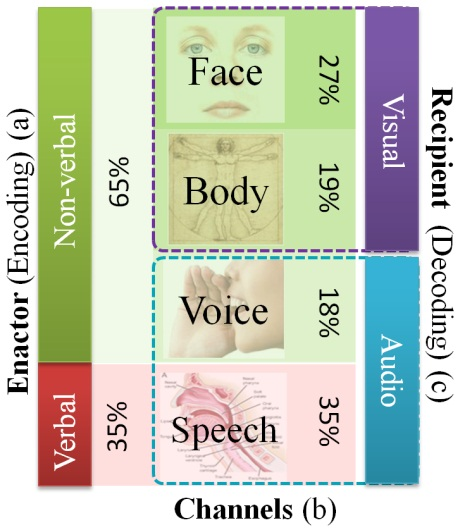
\includegraphics[width=3in]{NVCEncodings.jpg}
\end{center}
\caption{Relative importance of a) verbal vs. non-verbal cues, b) four channels of non-verbal cues, and c) visual vs. audio encoding and decoding of bilateral human interpersonal communicative cues.}
\label{Fig:Figure1}
\end{figure}

\subsubsection{Social Sight and Social Hearing}
Unlike speech, which is mostly under the conscious control of the user, the non-verbal communication channels are engaged from a subconscious level. Though people can increase their control on these channels through training, innately, individuals demonstrate certain inability to control their non-verbal cues. This inability to control non-verbal channels is referred to as the leakiness \cite{brown_social_1986} and humans (evolutionarily) have learnt to pick up these leaked signals during social interactions. For example, people can read very subtle body mannerisms very easily to determine the mental state of their interaction partner. Eye Gaze is a classic example of such subtle cues where interaction partners can detect interest, focus, involvement and role play, to name a few.  On this leakiness scale, it has been found that the voice is the leakiest of all channels, implying that emotions of individuals are revealed first in their voice before any of the other channels are engaged. The voice is followed by body, face and finally the verbal channel, speech. The leakiness is plotted on the abscissa of Figure \ref{Fig:Figure2} with the ordinate showing the amount of information encoded in the other three non-verbal communication channels. It can be seen that the face communicates the most amount of non-verbal cues, while the prosody (voice) is the first channel to leak emotional information.

\begin{figure}[h]
\begin{center}
 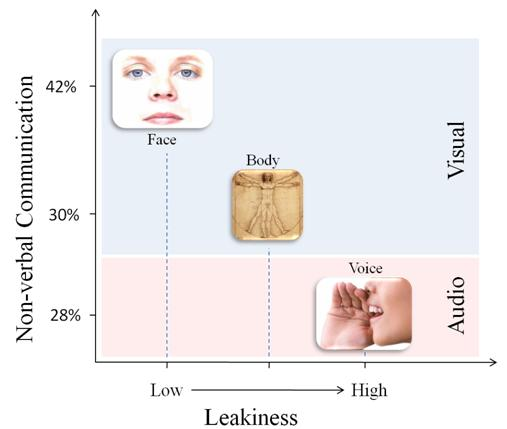
\includegraphics[width=4in]{Leakiness.jpg}
\caption{Relative communicative information plotted against its leakiness. Speech forms the verbal channel. Face, body and voice form the non-verbal communication channels.}
\label{Fig:Figure2}
\end{center}
\end{figure}

\subsubsection{Social Touch}
Apart from visual and auditory channels of social stimulation, humans increasingly rely on social touch during interpersonal interactions. For example, hand shake represents an important aspect of social communication conveying confidence, trust, dominance and other important personal and professional skills \cite{burgoon_relational_1984}. Social touch has also been studied by psychologists in the context of emotional gratification. Wetzel \cite{wetzel_midas_1984} demonstrated patron gratification effects through tipping behavior when waitresses touched their patrons. Similar studies have revealed the importance of social touch and how conscious decision making is connected deeply with the human affect system. In the recent years social touch has gained a lot of interest in the area enriching remote interactions \cite{haans_mediated_2006} \cite{bailenson_virtual_2008} to help better understand an individual's  social awareness and social presence. In the next section, we describe the term \emph{Social Situational Awareness} as seen pertinent to this report and emphasize the importance of any individual being aware of his/her social situational awareness.

\section{Social Situational Awareness}
We refer to the term Social Situational Awareness (SSA) as the ability of individuals to receive the visual, auditory and touch based non-verbal cues and respond appropriately through their voice, face and/or body (touch and gestures). Figure \ref{Fig:Figure3} represents the concept of consuming social cues and reacting accordingly to the needs of social interaction. Social cognition bridges stimulation and reciprocation and allows individuals to interpret and react to the non-verbal cues.

\begin{figure}[h]
\begin{center}
 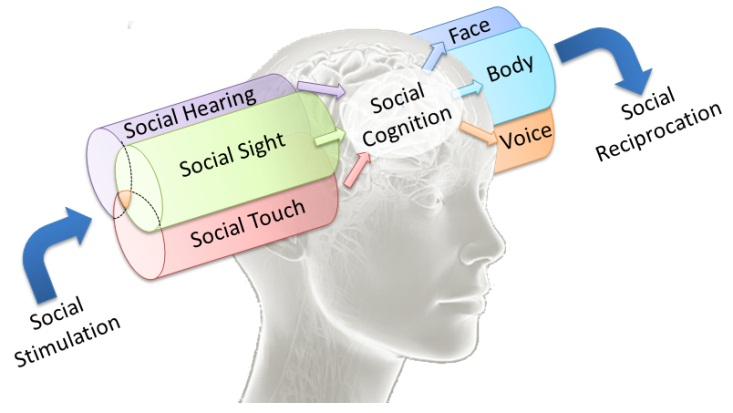
\includegraphics[width=4.5in]{SSA.jpg}
 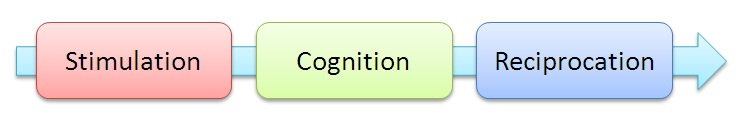
\includegraphics[width=4.5in]{SSA2.jpg}
\caption{Social Situational Awareness.}
\label{Fig:Figure3}
\end{center}
\end{figure}

The Transactional Communication Model \cite{sameroff_reproductive_1975} suggests that during any face-to-face interaction, the interpretation of the social stimulation and the corresponding social response are under the control of various factors including the culture, physical and emotional state, experience, memory, expectation, self concept and attitude of the individuals involved in the interaction. In order to effectively cognize and react to the social stimulation, it is necessary that individuals be able to receive and synthesize these above factors. Enriching social situational awareness then represents the ability of a mediator (telecommunication technology for remote interactions; social assistive technologies for the disabled population) to allow the social cognition of an individual to have access to the above mentioned factors and thereby evoking appropriate social reciprocation.

\subsection{Social Situational Awareness in Everyday Social Interactions}
\subsubsection{SSA in Dyadic Interactions}
Human communication theories have studied dyadic or bilateral interaction between individuals as the basis of most communication models. Theories of leadership, conflict and trust base their findings on dyadic interaction primitives where the importance of the various non-verbal cues is heightened due to the one-on-one nature of dyadic interactions. Eye contact, head gestures (nod and shake), body posture (conveying dominance or submissiveness), social touch (hand shake, shoulder pat, hug, etc.), facial expressions and mannerisms (smile, surprise, inquiry, etc.), eye gestures (threatened gaze, inquisitive gaze, etc.) are some of the parameters that are studied closely in dyadic understanding of human bilateral communication \cite{altmann_analysis_2007}. Enriching SSA in dyadic communication thus focuses on appropriate extraction and delivery of communicator's face, body and voice based behaviors to a remote participant or to a person who is disabled.

\subsubsection{SSA in Group Interactions}
Group dynamics refer to the interactions between members of a team assembled together for a common purpose. For example, teams of medical professionals operating on a patient, a professional team meeting for achieving a certain goal, a congressional meeting on regulations, etc. represent groups of individuals with a shared mental model of what needs to be accomplished. Within such groups, communication behaviors play a vital role in determining the dynamics and outcome of the meeting. Zancanaro et. al. \cite{zancanaro_automatic_2006} and Dong et. al.  \cite{dong_using_2007} presented one model of identifying role-play of participants in a group discussion. They identified two distinct categories of roles for the individuals within the group, namely, the socio-emotion roles and the task roles. The socio-emotional roles included the protagonist, attacker, supporter and neutral, and the task roles included the orienteer, seeker, follower and giver. These roles were dependent heavily on the emotional state (affect) of the individuals participating in the group interaction. Good teams are those where individual team members and their leaders are able to compose and coordinate their affect towards a smooth and conflict free group interaction. And effective leaders are those who can read the affect of their group member, make decisions on individual's roles and steer the group towards effective and successful decisions. Inability to access the affective cues of team members has significant consequences to team leaders leading to unresolved conflict situations and underproductive meetings, or in the worst case, the death of a patient. Thus, enriching SSA in group settings correspond to the extraction and delivery of team's interaction dynamics (which are in turn modulated in their mutual and group affect) to a remotely located team member or to a co-located individual who is disabled.

In essence, SSA enrichment technologies provide for a richer interaction experience for individuals involved either in a dyadic or group interaction. It is well established that in teams comprising of good communication strategies a shared mental model towards effective decision is achieved faster with little or no emotional stress on the team members. The lack of social awareness can lead to interactions where individuals are not committed cognitively and find it very difficult to focus their attention on the communication. This is true in the case of remote interactions, disability and situations where doctors, nurses and other medical professionals are operating simultaneously on a patient.

\subsection{Learning Social Awareness}
Figure \ref{Fig:Figure3} represents a simple unidirectional model of social stimulation and reciprocation. In reality, social awareness is a continuous feedback learning system where individuals are learning through observing, predicting, enacting and correcting themselves. It is this learning mechanism that allows people to adapt easily from one culture to another with ease - here we refer to term culture in very broadly encompassing work culture, social culture in a new environment and culture of a new team, etc. Figure \ref{Fig:Figure4} shows the continuous feedback loop involved in social learning systems, based on the model of human cognition as proposed by Hawkins \cite{hawkins_intelligence_2004}.

\begin{figure}[h]
\begin{center}
 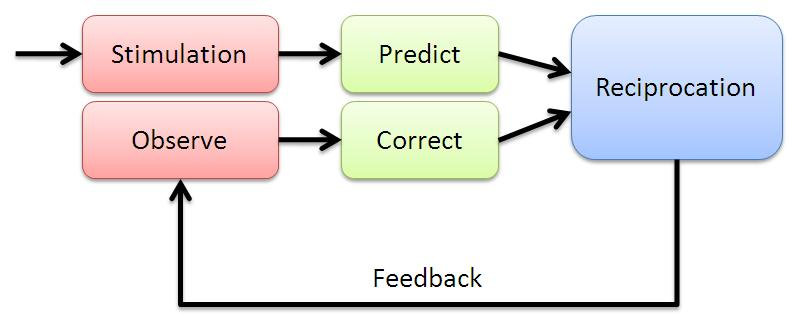
\includegraphics[width=4.5in]{SSALearning.jpg}
\caption{Social learning systems with continuous learning feedback loop.}
\label{Fig:Figure4}
\end{center}
\end{figure}

People exposed to everyday social interactions learn social skills from the three different social stimulations (social sight, social hearing and social touch) effortlessly. When faced with a new environment, individuals exercise their learned social skills to predict what social actions are appropriate in the setting. Once executed, they observe and assess their counterparts to determine if their new behavior is appropriate or not for the new setting. Such learning continues until their social rule set adapts to the new environment. Psychologists have been studying the nature of learning that happens in individuals who move from Western to Eastern cultures and vice versa. Largely, USA and Japan have been the countries of choice based on their economic equality and cultural diversity \cite{rogers_edward_2002}. In the West, large body movements and excitement in the voice are considered to be typical and to a large part encouraged as a good social skill. Similar attitudes in the East are considered to be inappropriate in professional settings and to a large extent considered indecent. An individual displaying any such inappropriate mannerisms or gestures will receive social feedback from his counterparts (everyone staring at the individual, reduced interaction with the individual, etc.).  Thus, social awareness is a learned set of rules about the environment within which the individual is present and this requires continuous monitoring of the various social channels of stimulation. Deprivation of any one of these channels can in turn affect the ability of the individual to learn social actions and responses that are pertinent to a social situation. Thus, enriching SSA not only offers the means for individuals to make appropriate social decisions, but also cognitively trains them towards effective social judgments.

-------------------------------------
In this paper, we advocate that the social separation induced by remote interactions in physically separated partners is similar to the social separation resulting from information impoverishment induced by sensory/physical disabilities in co-located interaction partners and propose technologies targeted at enriching social interactions.
--------------------------------------

\section{Components of Non-verbal Communication}
Non-verbal communications are inherently complex in nature. In order to understand the nature of these cues, psychologists have been studying these cues under three subdivisions based on what affects individual’s non-verbal cueing \cite{knapp_nonverbal_1996}. These subdivisions include,
\begin{enumerate}[(a)]
\item The communication environment
\item  The physical characteristics of the communicators
\item The behaviors of the communicators
\end{enumerate}
Below, these three items are discussed in detail providing a highlevel discussion on the nature of their influence on the non-verbal communication between individuals.

\subsection{The Communication Environment}
The communication environment or surroundings where the interactions are taking place make a huge difference of how humans respond or react \cite{hargie_social_1994} \cite{walsh_person-environment_2000}. For example, lengthy periods of extreme heat \cite{kenrick_ambient_1986} are known to increase discomfort, irritability, reduced work output and unfavorable evaluations of other. Along with the interaction partners, the environment either reinforces or depreciates the emotional experience of an individual. For example, wide open spaces and natural environments are known to be conducive for psychological stability \cite{krupat_people_1985}. Though the environmental factors just perceptual, they impose a lot of control on how humans react towards them. Some of the important environmental factors that affect interpersonal communication and non-verbal cueing are shown in the Table \ref{Tab:Tabel1}. **These are some of the well identified factors towards which psychologists and sociologists are working towards.**

\begin{table}[hpdf]
\begin{center}
\caption{The various factors of the communicator's environment that can affect interpersonal communication.}
\label{Tab:Tabel1}
\begin{tabular}{|l|l|}
\hline
\multicolumn{2}{|c|}{The Communication Environment} \\
\hline
Familiarity of the environment & \cite{sommer_personal_1969} \cite{sommer_tight_1974} \\
Colors in the environment & \cite{schauss_psysiological_1985} \cite{bottomley_interactive_2006} \\
Other people in the environment	& See next two subsections. \\
Architectural Designs & \cite{farrenkopf_university_1980} \\
Objects in the environment & \cite{moos_human_1985} \\
Sounds  & \cite{manusov_attribution_2001} \cite{north_-store_1997} \\
Lighting & \cite{meer_light_1985} \\
Temperature & \cite{kenrick_ambient_1986} \\
\hline
\end{tabular}
\end{center}
\end{table}

\subsection{The Physical Characteristics of the communicators}
The physical appearance of a person is very important aspect of non-verbal cueing. People draw impressions of their communication partner as soon as they see them. The human body acts like means for communicating important sociological parameters like status, interest, dominance etc. Researchers have found cultural and global preferences in overall body image and any deviations from the norm affects interactions between people. For example, facial babyishness \cite{berry_attractive_1991} has been found affect judgment of facial attractiveness, honesty, warmth and sincerity. Any deviation from the babyishness has been correlated to immediate reduction in the judgment of these traits. A similar such example is the clothing that people wear. It has been found that first impressions are positive if the interviewer and interviewee are clothed similarly \cite{johnson_clothing_1977}. Table \ref{Tab:Table2} shows the important aspects of a person's physical appearance that affects the interpersonal interaction. Various psychological studies have been conducted towards understanding the model of human perception of character. Very little is known on the reasons for some of the human norms, but it is an active area of research that is being explored rigorously, especially, in the context of group behaviors and personal mannerisms with work environments \cite{helen_h._jennings_sociometry_1959}.

\begin{table}[hpdf]
\begin{center}
\caption{The physical characteristics of a communicator that can affect interpersonal communications.}
\label{Tab:Table2}
\begin{tabular}{||l||l||}
\hline
\hline
\multicolumn{2}{||c||}{The Physical Characteristics} \\
\hline
\hline
The human facial attractiveness	& \cite{berry_attractive_1991} \cite{zebrowitz_reading_1997} \cite{berry_perceiving_1986}\\
\hline
Body shape & \cite{cortes_physique_1965} \cite{tucker_physical_1984}\\
\hline
Height of a person & \cite{cameron_courtship_1977}\\
\hline
Self image & \cite{ogden_prevalence_2002}\\
\hline
Body color & \cite{griffin_black_1996}\\
\hline
Body smell & \cite{porter_olfaction_1998} \cite{lord_identification_1989} \cite{russell_human_1976}\\
\hline
Body hair & \cite{barber_mustache_2001}\\
\hline
Clothing & \cite{johnson_clothing_1977} \cite{hensley_effects_1981}\\
\hline
Personality	& \cite{joseph_uniforms_1986} \cite{rosenfeld_clothing_1977}\\
\hline
Body decoration or artifacts & \cite{sanders_customizing_2008}\\
\hline
\hline
\end{tabular}
\end{center}
\end{table}

\subsection{Physical Characteristics that affect interpersonal communication}
\subsubsection{Behavior of the Communicator}
The last of the three units of non-verbal communication is the behavior of the communicators. While the term behavior is used loosely in defining this unit, this encompasses both static posture and dynamic movements demonstrated by communicators. Of the three units of non-verbal communication, the behavior forms the most important aspect. Most part of the emotional information encoded by humans is delivered through the behavior of individuals during social interactions. Gestures, Posture, Touch and Voice form the basic subdivisions in behavioral non-verbal cueing. While the entire human body is important for the communication of these cues, the face and eyes play a major role.

\subsubsection{Gesture}
Gestures are dynamic movement of face and limbs displayed during interpersonal communication. Together, they convey a lot of information that is sometimes redundant (with speech) while other times deliver emotional information about the enactor. Most often gestures are classified based on their occurrence with speech. Accordingly, there are
\begin{enumerate} [(a)]
\item Speech-independent gestures, or emblems (like shrug, thumbs up, victory sign etc), that are mostly visual in nature and convey the user's response to the situation \cite{ekman_nonverbal_1976} \cite{wagner_field_2003}.
\item Speech-related gestures, or illustrators (pointing to a thing, drawing a shape while describing etc) \cite{efron_gesture_1972}.
\item Punctuation gestures, that emphasize, organize and accent important segments of a communication, like pounding the hand, raising a fist in the air etc.
    \end{enumerate}

\subsubsection{Posture}
Posture refers to the temporary limb and body positions assumed by individuals during interpersonal interactions.  Posture is a very effective medium for communicating some of the important non-verbal cues like leadership, dominance \cite{weisfeld_erectness_1982}, submissiveness and social hierarchy \cite{grant_comparison_1963}. For example, people who show a tendency of dominance tend to extend their limbs out while sitting thereby displaying an overall larger body size. Similarly, submissiveness seems to be correlated to reducing the overall body size by keeps the limbs together.

Both gestures and postures are influenced heavily by the cultural background of the individual and also varied with the geographical location \cite{kleinsmith_cross-cultural_2006}. Though the cultural influence if true with other non-verbal and verbal cues, the perceived difference is the highest in gestures and posture displayed by individuals.

\subsubsection{Touch}
Social touch has been a very important aspect of non-verbal communication in humans. Developmental biologists believe that the first set of sensory responses in a human fetus is touch \cite{montagu_touching:_1986}. From a social context this sensory channel is very well used in conveying important interpersonal cues such as interest, intimacy, warmth, confidence, leadership and sympathy \cite{afifi_use_1999}. Touch is a powerful means of unconscious interaction and it is believed that people who are very good in their social skills rely upon touch a lot \cite{hertenstein_communicative_2006}. Historically, the sense of touch (Haptics Communication \cite{hertenstein_touch_2006}) has been studied by psychologists in the perspective of understanding the human sensory system, but recently, haptics has grown out into the technology front providing human machine interfaces that augment or replace visual and auditory interfaces \cite{robles-de-la-torre_principles_2008}.

\subsubsection{Face}
The face is the primary channel for non-verbal communication. Humans are efficient in conveying and receiving plethora of information through subtle movements of their face and head. This focus on the face develops from a very young age and it has been shown that by 2 months, infants are adept in understanding facial gestures and mannerisms \cite{carver_development_2002}. The human face has very fine muscular control allowing it to perform complex patterns that are common to humans, while at the same time being vastly individual \cite{rinn_neuropsychology_1984}. The facial appearance of an individual is due to their genetic makeup, transient moods that stimulate the facial muscles and due to chronically held expressions that seem to set in and become permanent. Human visual system has developed the ability to read these subtleties on people's faces and interpret all the three aspects of the face - genetic makeup (person's identity through face recognition), transient mood (facial expression and emotion recognition), and permanent expression on the face (default neutral face of individuals). While the aspects of permanent facial appearance are important in the recognition of the individual, from a non-verbal communication perspective, the primary function of the face is directed towards communicating emotions and expressions.

The understanding of the human facial expression space was immensely increased by the work of Ekman, Frisen \cite{ekman_facial_1978} and Izard \cite{izard_maximally_1983} in the late 1970s. They independently measured precise facial movement patterns and correlated these individual movements with facial expressions on the human face. While Izard developed these patterns on infants, the Facial Action Coding System (FACS) developed by Ekman and Frisen has become the de facto standard for measuring facial expressions and emotions. FACS allow expression and emotion researchers to encode facial movements into accurate contraction and relaxation of facial muscles. Based on these facial actions, Ekman and Frisen discovered the global occurrence of seven basic judged emotions. As psychologists have started to master the FACS system of analyzing facial actions, human computer interaction specialists have started to use the same FACS encodings for building better interfaces that can determine human affect and respond accordingly.

\emph{Facial Action Coding System (FACS):}
FACS defines all possible facial feature movements into Action Units (AU) which represent movement of facial features (like lips, eye brow, chin etc). The AUs are the net effect of facial muscle contraction and relaxation, though they are not directly related to the muscles. Table below shows the different AUs that form the basis of FACS based facial coding with the appropriate number and the associated facial feature movement.

\begin{table}[hpdf]
\begin{center}
\caption{FACS communicative actions on the human face}
\label{Tab:Table2}
\begin{tabular}{|l|l||l|l|}
\hline
1 & Inner Brow Raiser & 24 & Lip Pressor\\
2 & Outer Brow Raiser & 25 & Lips part\\
4 & Brow Lowerer & 26 & Jaw Drop\\
5 & Upper Lid Raiser & 27 & Mouth Stretch \\
6 & Cheek Raiser & 28 & Lip Suck\\
7 & Lid Tightener & 29 & Jaw Thrust \\
9 & Nose Wrinkler & 30 & Jaw Sideways \\
10 & Upper Lip Raiser & 31 & Jaw Clencher\\
11 & Nasolabial Deepener & 32 & Lip Bite \\
12 & Lip Corner Puller & 33 & Cheek Blow \\
13 & Cheek Puffer & 34 & Cheek Puff \\
14 & Dimpler & 35 & Cheek Suck \\
15 & Lip Corner Depressor & 36 & Tongue Bulge \\
16 & Lower Lip Depressor & 37 & Lip Wipe\\
17 & Chin Raiser & 38 & Nostril Dilator \\
18 & Lip Puckerer & 39 & Nostril Compressor\\
19 & Tongue Out & 41 & Lid Droop \\
20 & Lip stretcher & 42 & Slit\\
21 & Neck Tightener & 43 & Eyes Closed\\
22 & Lip Funneler & 44 & Squint\\
23 & Lip Tightener & 45 & Blink\\
& & 46 & Wink\\
\hline
\end{tabular}
\end{center}
\end{table}

\subsubsection{Eye}
Like the human face, eyes are very important for the control of non-verbal communication. This involvement of human eyes comes from the functions that gaze and mutual gaze play in everyday human interpersonal communication \cite{argyle_gaze_1976}. People use their gaze to convey subtle information that enables smooth verbal interaction which eventually leads to information exchange \cite{kleinke_gaze_1986}. From a research perspective, the function of gaze has been classified into four important functional categories \cite{kendon_functions_1967}. These include

\begin{table}[hpdf]
\begin{center}
\caption{The role of human eye in interpersonal communications.}
\label{Tab:Table4}
\begin{tabularx}{5.5in}{|X|X|}
\hline
Regulating the flow of communication & One of the most important functions of gaze is the regulation of verbal communication in bilateral and group communications. People use gaze to shift focus, bring the attention of a group of people to one thing, turn taking in group conversations \cite{mast_dominance_2002} and eliciting response from communication partners \cite{bavelas_listener_2002}. \\
\hline
Monitoring feedback & Gaze provides a means for individuals to get feedback during conversations and communications. Feedback is a very important tool while people converse. Humans study the eyes of the listener to cognitively inject or eliminate more verbal information into the conversation \cite{van_dulmen_shifts_1997}. \\
\hline
Reflective of cognitive activity & Both listeners and speakers tend not to gaze at others when they are processing complex ideas or tasks. Studies have shown that people can answer better when they close their eyes and are allowed to process their thoughts \cite{glenberg_averting_1998}. Thus, cognitive processing is displayed very elegantly by monitoring eye gaze patterns. \\
\hline
Expressing emotions & Along with the facial muscular movements, the eyes play a vital role in the expression of emotions. In fact, in human computer interaction research, it has been found that relying on the eyes and the eyelids alone can provide more accurate delivery of affect information when compared to the entire face \cite{orozco_confidence_2008}. Verbal communication tends to move the lips and mouth quickly and randomly that can make image and video processing of expressions very tough. Some of the more recent spontaneous expression recognition research is focusing on the eyes for this very reason. \\
\hline
\end{tabularx}
\end{center}
\end{table}



\chapter{MOTIVATION}
\DoubleSpacing
\setlength{\parindent}{.5in}
In this chapter we discuss three important problems that highlight the need to communicate social situational awareness to individuals involved in interpersonal interactions.

\section{Assistive Technology}
most part of the non-verbal encoding happens through visual media. While some parts of these cues are delivered along with speech, most part of the nonverbal communication is inaccessible to someone with visual impairment or blindness. This disconnect from the visual stimulations deprive the individuals of vital communicative cues that enrich the experience of social interactions.  People who are blind cannot independently access this visual information, putting them at a disadvantage in daily social encounters.  For example, during a group conversation it is common for a question to be directed to an individual without using his or her name-instead, the gaze of the questioner indicates to whom the question is directed. In such situations, people who are blind find it difficult to know when to speak because they cannot determine the direction of the questioner's gaze. Consequently, individuals who are blind might be slow to respond or talk out of turn, possibly interrupting the conversation. As another example, consider that people who are blind cannot use visual cues to determine when their conversation partners change positions (e.g., pacing the floor or moving to a more comfortable chair). In this scenario, an individual who is blind might inadvertently create a socially awkward situation by speaking in the wrong direction.

To compound these problems, sighted individuals are often unaware of their non-verbal cues and often do not (or cannot) make appropriate adjustments when communicating with people who are blind. Also, people who are blind often do not feel comfortable asking others to interpret non-verbal information during social encounters because they do not want to burden friends and family.  The combination of all these factors can lead people who are blind to become socially isolated \cite{segrin_poor_2000}, which is a major concern given the importance of social interaction. While people who are blind and visually impaired face a difficulty in social interactions, research in rehabilitation training for these populations recommends that the social involvement for these individuals have to substantially increase in order to enable their acceptance of the society.

National Center for Health Statistics reported in $2007$ that the estimated number of visually impaired and blind people totals up to $21.2$ million in the United States alone . Global numbers are daunting. In $2002$ more than $161$ million people were visually impaired, of whom $124$ million people had low vision and $37$ million were blind . World Health Organization reports that more than $82$\% of the populations who are blind or visually impaired are of age $50$ or older. With the life expectancy going up in most developing countries, the percentage of general population entering into some sort of visual impairment is going to increase in the coming years.

Recently, Jindal-Snape \cite{jindal-snape_generalization_2004} \cite{jindal-snape_use_2005} \cite{jindal-snape_using_1998} carried out extensive research in understanding social skill development in the blind and visually impaired. She has studied individual children (who are blind) from India where the socio-economic conditions do not provide for trained professionals to work with children with disabilities. Her seminal work in understanding social needs of children who are blind have revealed two important aspects of visual impairment that restricts seamless social interactions.

While most persons who are blind or visually impaired eventually make accommodations for the lack of visual information, and lead a healthy personal and professional life, the path towards learning effective accommodations could be positively effected through the use of assistive aids. Specifically, children with visual disabilities find it very difficult to learn social skills while growing amongst sighted peers, leading to social isolation and psychological problems \cite{jindal-snape_generalization_2004}. Social disconnect due to visual disability has also been observed at the college level \cite{shinohara_blind_2009} where students start to learn professional skills and independent living skills. Any assistive technology aid that can enrich interpersonal social interactions could prove beneficial for persons who are visual disabled.

\section{Remote Interactions}
An industry survey \cite{solomon_challenges_2010} of $1592$ individuals who collaborated remotely, carried out by RW3 CultureWizard - a company focused on improving international collaborations - reported difficulties similar to what was faced by the individuals who are blind. "Respondents found virtual teams more challenging than face-to-face teams in managing conflict ($73$\%), making decisions ($69$\%), and expressing opinions ($64$\%). The top five challenges faced during virtual team meetings were insufficient time to build relationships ($90$\%), speed of decision making ($80$\%), different leadership styles ($77$\%), method of decision making ($76$\%), and colleagues who do not participate ($75$\%)." These results can be correlated to the need for Social Situational Awareness in group settings, specifically one that can promote leadership and personal understanding of each other as indicated in Section 2.1.2.

Further, when the participants were asked about the personal challenges faced during virtual team meetings, they reported inability to read non-verbal cues ($94$\%), absence of collegiality ($85$\%), difficulty establishing rapport and trust ($81$\%), difficulty seeing the whole picture ($77$\%), reliance on email and telephone ($68$\%), and a sense of isolation ($66$\%)." Delivering non-verbal cues, establishing trust and rapport, and easing isolation are all derivatives of increasing one's social connection to their interaction partners, be it remote or face-to-face. Observing people who are disabled and the way they communicate with their co-located partners, it is possible to derive inspirations for novel social mediation technologies. The following subsection discusses one example of how to develop an evidence-based social situational awareness model based on hand shaking in the blind population as an example of social interaction between participants.

\begin{table}
\caption{Survey on the challenges of remote interaction \cite{solomon_challenges_2010}}
\label{Table:Tab3}
\begin{tabular}{|l|}
\hline
Challenges in virtual teams compared to face-to-face teams \\
\hline
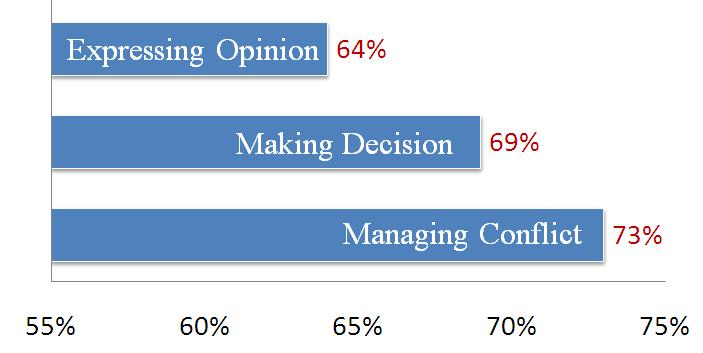
\includegraphics[width=3in]{Suggestion1.jpg}\\
\hline
Top five challenges faced during virtual team meetings \\
\hline
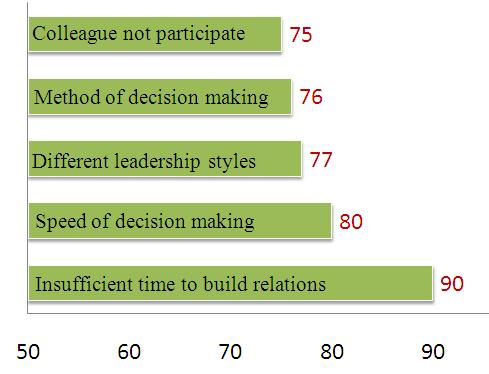
\includegraphics[width=3in]{Suggestion2.jpg}\\
\hline
Personal challenges during virtual team meetings\\
\hline
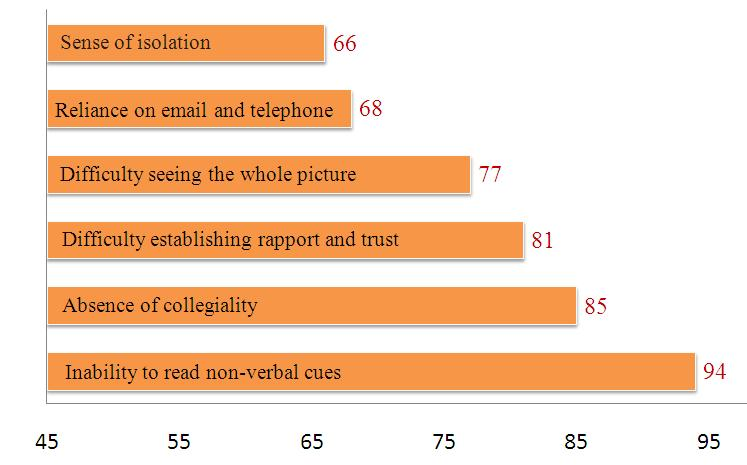
\includegraphics[width=4.5in]{Suggestion3.jpg}\\
\hline
\end{tabular}
\end{table}





\section{Medical Teams}






\chapter{ASSISTIVE TECHNOLOGY DESIGN}

\DoubleSpacing
\setlength{\parindent}{.5in}
Affective Computing research has employed algorithmic framework to quantitatively study both verbal and non-verbal cues displayed by the humans during social communication.  Signal streams from various sensors, including visual sensors (e.g. cameras), audio sensors (e.g. microphones) and various physiological sensors (such as EEG, EMG, and galvanic skin resistance sensors) have been used to evaluate human emotional states.  A good review of research work in Affective Computing can be found in \cite{zhihong_zeng_survey_2009}.  This research has enabled a better understanding of human physiological signals, with respect to emotional states, and the results have been used to facilitate human-computer interaction (HCI). In theory, a system that can detect non-verbal social cues could also be used as an assistive device to provide social feedback to people with disabilities.  The emphasis here would not be so much on interpreting these cues as on presenting social cue information to the user, and allowing the user to interpret them.  However, very little research has been done towards finding intuitive methods for presenting social cue information to humans.  \cite{ur_rehman_manifold_2007} developed a haptic chair for presenting facial expression information.  It was equipped with vibrotactile actuators on the back of the chair that represented some specific facial feature. Experiments conducted by the researchers showed that people were able to distinguish between six basic emotions.  However, this solution had the obvious limitation that the user needed to be sitting in the chair to use the system.

\emph{Observation 1: Assistive technology designed towards social assistance should be portable and wearable so that the users can use them at various social circumstances without any restriction to their everyday life.}

People with disabilities are not always able to perceive or interpret implicit social feedback as a guide to improving their communication competence.  However, they might be able to use explicit feedback provided by a technological device.  Rana and Picard \cite{teeters_self-cam:_2006} developed a device called Self Cam, which provides explicit feedback to people with Autism Spectrum Disorder (ASD).  The system employs a wearable, self-directed camera that is supported on the users own shoulder to capture the user's facial expressions. The system attempts to categorize the facial expressions of the user during social interactions to evaluate the social interaction performance of the ASD user.  Unfortunately, the technology does not take into account the social implication of assistive technologies. Since the technology is being developed to address social interactions, it is important to take into account the social artifacts of technology. A device that has unnatural extensions could become more of a social distraction for both the participants and users than as an aid.


\emph{Observation 2: Assistive technology designed towards social assistance should allow seamless and discrete embodiment of sensors or actuators making sure the device does not become a social distraction.}

Vinciarelli et. al. \cite{vinciarelli_social_2008} have described the use of discrete technologies for understanding social interactions within groups, specifically targeting professional environments where individuals take decisions as a group. They analyze the use of bodily mannerisms and prosody to extract nonverbal cues that allow group dynamics analysis. They rely on simple sensors in the form of wearable tags \cite{kim_meeting_2008} which detect face to face interaction events along with prosody analysis to determine turn taking, emotion of the speaker, distance to an individual etc. Pentland describes these signals captured during group interactions as \cite{pentland_honest_2008} honest signals. Some of his recent works \cite{vinciarelli_social_2008-1} in the area of social monitoring hopes to capture these signals and provide feedback to individuals about their social presence within a group. The use of social feedback is illustrated elegantly in their work but their findings relied on sensors carried by all individuals involved in the study. Having everyone in a group wear sensors has proved to be a viable and productive approach for studying group dynamics.  However, this approach is not viable as a strategy for developing an assistive technology, as it is not realistic to assume that everyone who interacts with a person with a disability will wear sensors.

\emph{Observation 3: Assistive technology designed towards social assistance should incorporate mechanisms embodied on the user to determine both self and other's social mannerism.}

In two independent experiments \cite{transon_using_1988} and \cite{felps_modification_1988}, researchers developed a social feedback device that provides intervention when a person with visual impairment starts to rock their body displaying a stereotypy. \cite{transon_using_1988} designed a device that consisted of a metal box with a mercury level switch that detects any bending actions. The feedback was provided with a tone generator that was also located inside the metal box.  The entire box was mounted on a strap that the user wears around his/her head. The authors tested it on a congenitally blind individual who had severe case of body rocking and they conclude that the use of any assistive technology is useful only temporarily while the device is in use. They state that the body rocking behavior returned to baseline levels as soon as the device was removed. Since the time of this experiment, behavioral psychology studies have explored short term feedback for rehabilitation \cite{jindal-snape_use_2005}, and these studies support the above observation that short term feedback is often detrimental to rehabilitation and subject's case invariably worsens. Unfortunately, due to the prohibitively large design of the device developed by these researchers, it was impossible to have the individual wear the device over long durations.

\emph{Observation 4: Assistive technology designed towards social assistance and behavioral rehabilitation should be used over long durations in such a way that the feedback is slowly tapered off over a significantly longer duration of time.}


In \cite{felps_modification_1988} researchers used a 'Drive Alert' (driver alerting system that monitors head droop) to detect body rocking and provide feedback to a congenitally blind 21 year old student. The research concludes that they were able to control body rocking effectively, but the device could not differentiate between body rocks from any other functional body movements. This device, primarily built to sense drooping in drivers provides no opportunity to differentiate between a body rock and a functional droop. Use of such devices could only be negative on the user as a large number of false alarms would only discourage an individual from using any assistive technology.

\emph{Observation 5: Assistive technology designed towards social assistance and behavioral rehabilitation should be effective in discriminating social stereotypic mannerisms from other functional movements to keep the motivation of device use high.}


\section{Conceptual Framework}
\subsection{Design principles for social assistive and rehabilitative devices}
A device that is developed to facilitate the social interactions of people with sensory, or cognitive disabilities might do so by, (a) detecting social cues during social interactions and delivering that information to the user in real time to enable empathy, or (b) detecting the user's stereotypic behaviors during social interactions and communicating that information to the user in real time to provide social feedback.  The first device might be classified as an assistive technology, while the second might be classified as a rehabilitative technology.  Ideally, such a device would be based on the following design principles:

\begingroup
\leftskip0.5in
\setlength{\parindent}{0in}
\emph{Design principle 1:} The device should be portable and wearable so that it can be used in any social situation, and without any restriction on the user's everyday life.

\emph{Design principle 2:} The device should employ sensors and personal signaling devices that are unobtrusive, and do not become a social distraction.

\emph{Design principle 3:} The device should include sensors that can detect the social mannerisms of both the user and other people with whom the user might communicate.

\emph{Design principle 4:} The device should be comfortable enough to be worn repeatedly for extended periods of time, to allow it to be used effectively for rehabilitation.

\emph{Design principle 5:} The device should be able to reliably distinguish between the user's problematic stereotypic mannerisms and normal functional movements, to ensure that it will be worn long enough to achieve rehabilitation.

\endgroup

\section{Requirements Analysis for a Social Assistive Technology for Individuals who are Blind and Visually Impaired}
In order to identify the unmet needs of the visually impaired community, two focus groups consisting primarily of people who are blind, as well as disability specialists and parents of students with visual impairment and blindness where conducted \footnote{ In  order  to  understand  the  assistive  technology  requirements  of  people  who  are  blind, we conducted two focus group studies (one in Tempe, Arizona USA - $9$ participants, and another in Tucson, Arizona USA - $11$ participants) which included:
\begin{enumerate}[1.]
\item Students and adult professionals who are blind,
\item Parents of individuals who are blind
\item Professionals who work in the area of blindness and visual impairments.
\end{enumerate}
There was unanimous agreement among participants that a technology that would help people with visual impairment to recognize people or hear them described would significantly enhance their social life.}. Members of these focus groups who were blind or visually impaired were encouraged to speak freely about their challenges in coping with daily living. During these focus groups, the participants agreed on many issues as being important problems. However, one particular problem - that of engaging freely with their sighted counterparts - was highlighted as a particularly important problem that was not being addressed by technology specialists \footnote{  To quote some candidate's opinion about social assistance technology in a everyday setting:
\begin{itemize}
\item \"It would be nice to walk into a room and immediately get to know who are all in front of me before they start a conversation\".
\item One young man said, \"It would be great to walk into a bar and identify beautiful women\".
\end{itemize}}.

While various other examples were cited by individuals during these focus group studies, the inability to access non-verbal cues were considered of highest priority. Based on these discussions, a list of needs was complied that characterized social needs often experienced by people with visual impairments. In doing so, two important aspects of social interaction were identified. These included
\begin{enumerate}[1.]
\item Access to the non-verbal cues of others during social interactions, and
\item How one is perceived by others during social interactions.
\end{enumerate}

These needs correlated with the psychology studies conducted by Jindal-Snape with children who were visually impaired. She identifies these two needs under the \emph{Social Learning} and \emph{Social Feedback}. While these two important categories were identified, for simplification, the non-verbal cue needs were reduced to $8$ aspects of social interactions that focused primarily on the physical characteristics of the interaction partner and the behaviors of the
interaction partner. These questions were developed with the help of visually impaired professionals and students:

\begin{enumerate}[1.]
\item Knowing how many people are standing in front you, and where each person is standing.
\item Knowing where a person is directing his/her attention.
\item Knowing the identities of the people standing in front of you.
\item Knowing something about the appearance of the people standing in front of you.
\item Knowing whether the physical appearance of a person who you know has changed since the last time you encountered him/her.
\item Knowing the facial expressions of the person standing in front of you.
\item Knowing the hand gestures and body motions of the person standing in front of you.
\item Knowing whether your personal mannerisms do not fit the behavioral norms and expectations of the sighted people with whom you will be interacting.
\end{enumerate}

Further, in order to understand the importance of these non-verbal communication primitives an online survey was carried out to determine a self-report importance map of the various non-verbal cues. This list of questions included both the importance from the perspective of allowing access to the non-verbal cues of the interaction partner (for enabling Social Learning), while also focusing on the personal body mannerism (for enabling Social Feedback) of the individual.The online survey was anonymously completed by $28$ people, of whom $16$ were blind, $9$ had low vision, and $3$ were sighted specialists in the area of visual impairment and vocational training. The online survey consisted of eight questions that corresponded to the previously identified list of needs. Respondents answered each question using a Five-point Likert scale, the metrics being (1) Strongly disagree, (2) Disagree, (3) Neutral, (4) Agree, and (5) Strongly agree.

\section{Results from the Online Survey}
\subsection{Average Response}
Table \ref{Tab:Table5} shows the eight aspects of social interactions that were investigated with the individuals who are blind and visually impaired. The results are sorted by descending importance, as indicated by the survey respondents (the question numbers correspond to the need listed in the previous section). The mean score is the average of the respondents on the $5$ point scale that was used to capture the opinions.  A score closer to $5$ implies that the respondents strongly agree with a certain question and that they consider inaccessibility to that particular non-verbal cue to be important deterrent to their social interactions. On the other hand, a score closer to $1$ represents the respondent did not consider the access to a specific non-verbal cue to be important during their social interactions.

\begin{table}[h]
\caption{Average Score on the 8 Questions obtained through an Online Survey.}
\label{Tab:Table5}
\begin{center}
\begin{tabularx}{5in}{|l|X|c|}
\hline
Question No. & Question & Mean Score\\
\hline
8. & I would like to know if any of my personal mannerisms might interfere with my social interactions with others. & 4.5 \\
\hline
6. & I would like to know what facial expressions others are displaying while I am interacting with them. & 4.4 \\
\hline
3. & When I am standing in a group of people, I would like to know the names of the people around me. & 4.3 \\
\hline
7. & I would like to know what gestures or other body motions people are using while I am interacting with them. & 4.2 \\
\hline
1. & When I am standing in a group of people, I would like to know how many people there are, and where each person is. & 4.1 \\
\hline
2. & When I am standing in a group of people, I would like to know which way each person is facing, and which way they are looking. & 4.0 \\
\hline
5. & I would like to know if the appearance of others has changed (such as the addition of glasses or a new hair-do) since I last saw them. & 3.5 \\
\hline
4. & When I am communicating with other people, I would like to know what others look like. & 3.4 \\
\hline
\end{tabularx}
\end{center}
\end{table}

\subsection{Response on Individual Questions}
Figure \ref{Fig:Figure6} shows the histogram of responses for the 8 Questions that were asked as part of the survey. Each subplot refers to a single question and shows the number of times users responded to that particular question with answers from 1 to 5 on the Lickert Scale. Each histogram adds up to a total of 28 that corresponds to the 28 participants that took part in the online survey.

\begin{figure}[h]
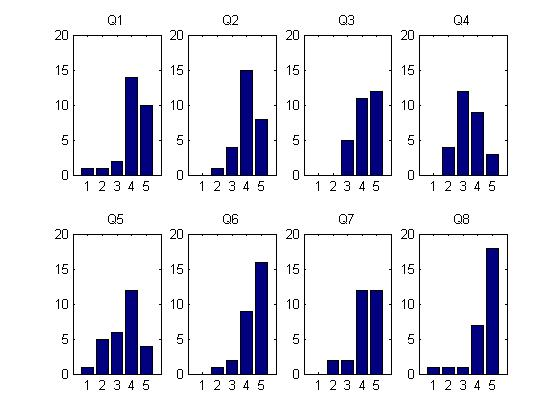
\includegraphics[width=5.5in]{histogram.jpg}
\caption{Histogram of Responses grouped by Questions}
\label{Fig:Figure6}
\end{figure}

Some of the observations from the important histograms include,
\begin{itemize}
\item Respondents are highly concerned about how their body mannerisms are perceived by their sighted peers (based on the response to Question 8 on the survey).
\item Facial expressions form the most important visual non-verbal cue that individuals who are blind or visually impaired feel they do not have access to (based on Question 6 on the survey). This correlates with the studies into non-verbal communication that highlights the importance of facial mannerisms and gestures, which are mostly visual in their decoding.
\item Followed by facial expressions, body mannerisms seem to be of higher importance for individuals who are blind and visually impaired (based on Question 3 of the survey).
\item The responses to questions 7, 1 and 2 suggest that respondents would like to know the identities of the people with whom they are communicating, relative location of these people and whether their attentions are focused on the respondent. This corresponds to knowing the position of their interaction partners when they are involved in a bilateral or group communication. People tend to move around, especially when they are standing, causing people who are blind to lose their bearing on where people were standing. This can result in individuals addressing an empty space assuming that someone was standing there based on their memory.
\item The responses to questions 4 and 5 indicate that there was a wide variation in respondents' interest in (4) knowing the physical appearance of people with whom they are communicating and (5) knowing about changes in the physical appearance of people with whom they are communicating. Many respondents indicated moderate, little, or no interest in either of these areas.
\end{itemize}

\subsection{Response Ratio}
Figure \ref{Fig:Figure7} shows the number of times the respondents chose to answer the 8 questions with their agreement or disagreement. The y-axis has been normalized to 100 points. The graph shows that respondents chose to answer the most by agreeing (Likert Scale 4) with the 8 questions. Followed closely behind was the strong agreement (Likert Scale 5) with the questions asked in the survey. The respondents chose to answer the least through strong disagreement (Likert Scale 1) to what was asked in the survey.

\begin{figure}
\begin{center}
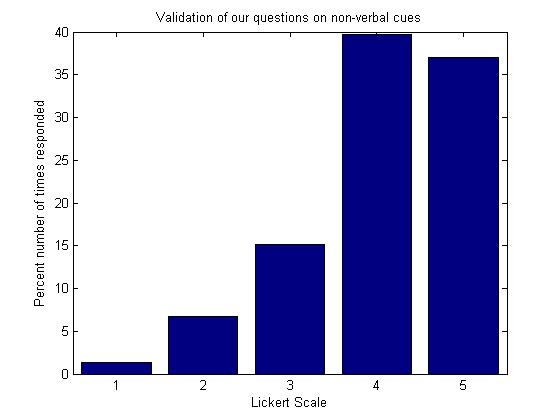
\includegraphics[width=5in]{responseratio.jpg}
\caption{Response Ratio}
\label{Fig:Figure7}
\end{center}
\end{figure}

As described earlier, the 8 questions corresponding to the social needs of the individuals were identified from the focus group survey that was conducted. Thus, the questions presented in the online survey questions were biased towards the needs of everyday social interactions of individuals who are blind and visually impaired. Thus, the implicit assumption while preparing this survey itself is that most of these items have been identified as being important and that only a priority scale needs to be extracted. This implicit assumption is immediately brought out by looking at the frequency with which the respondents answer with their agreement (Likert Scale 4) and strong agreement (Likert Scale 5).

\subsection{Rank Average Importance Map for Various Non-verbal Cues}
As can be seen from Figure \ref{Fig:Figure7}, the questionnaires were biased and the frequency of the responses is not Gaussian. This bias implies that using sample mean of the Lickert Scale responses will immediately show the same bias. This is due to the Gaussian iid assumption that is made while extracting the mean for the answers. In order to overcome this non-Gaussianity, we resort to non-parametric mean for the responses. Rank average of the responses is estimated instead of the typical mean of the responses for each of the question. Please see Appendix \ref{AppendixA} for the algorithm to determine the Rank Average. Since no assumptions on the distribution of the response are made, unlike the mean, the rank average gives a non-parametric method for comparing the responses of the individuals. The ranks can be either assigned ascending or descending with respect to the responses, i.e. rank 1 could mean all responses that were answered with strongly disagree (numeral 1), or rank 1 could mean all responses that were answered with strongly agree (numeral 5).

\begin{figure}
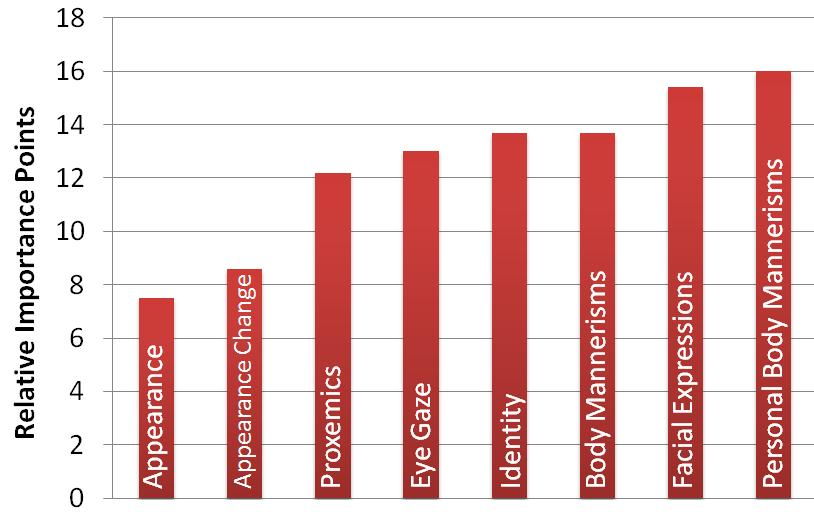
\includegraphics[width=5in]{rankaverage.jpg}
\caption{Rank average of the 8 questions}
\label{Fig:Figure8}
\end{figure}


In the Figure \ref{Fig:Figure8}, we have assigned rank 1 to strongly disagree. This is for the sake of visual convenience. Thus, higher the average rank, higher is that group's response from the respondents. Comparing Figure \ref{Fig:Figure8} to Table \ref{Tab:Table5}, it can be seen that the same ordering of priority can be seen through mean and rank average. But the mean tends to show very little variation between responses due to the bias that is present in the questions. On the other hand the rank average provides a good comparison scale.




%\newpage
\vspace*{1in}
%\chapter*{REFERENCES\hfill} \addcontentsline{toc}{chapter}{REFERENCES}
\begin{SingleSpace}
\bibliographystyle{ieeetr}	
\bibliography{references}
\end{SingleSpace}
%\clearpage

%% maybe endnotes
%% maybe bibliography
% if appendices, then

\appendix
\addcontentsline{toc}{chapter}{APPENDIX}
\chapter{\uppercase{Algorithm for Estimating Rank Average of Groups}}
\label{AppendixA}
\clearpage
While analyzing the responses of participants to the online survey, the participants responses for each question are represented as entries $x_{i,q}$, where, $i$ represents the $i^{th}$ participant and $q$ represents the $q^{th}$ question. $i = 1,\ldots,N$ are the $N$ participants who responded on the survey, and $q = 1, \ldots, Q$ are the $Q$ questions. In the survey presented in Chapter XXX, $N = 28$ and $Q = 8$.

\subsection{Procedure}

\begingroup
\setlength{\parindent}{0in}
\emph{Input:} Each participants response is considered as an entry $e_m$ into a pool $E = \{x_{i,q}\}$, where, $m=1,\ldots,M$, and $M=N$x$Q$. \\ \\
\emph{Ouput:} The rank average for the $Q$ groups (questions), $\bar{R}_m$.\\ \\
\emph{Steps:}
\begin{enumerate}[1.]
\item Group $e_n \in E$ removing all group affiliations.
\item Order the entries from $1$ to $M$ and assign a rank $r_{iq}$.
\item Assign any tied values the average of the ranks they would have received had they not been tied.
\item Rank Average for each group is then given as
\begin{equation}
\bar{R}_m = \frac{\displaystyle\sum\limits_{i \in Q_m, q=m}r_{iq}}{n_m}
\end{equation}
Where, $Q_m$ represents the group $m$ with the cardinality $n_m$. 
\end{enumerate}
\endgroup

Since no assumptions on the distribution of the response are made, unlike the mean, the rank average gives a non-parametric method for comparing the grpoups.

\chapter{\uppercase{Insert Appendix B Title here}}
\clearpage

% if Biographical sketch then
%\newpage
%\newpage
%\begin{center}\bibname\end{center} \addcontentsline{toc}{chapter}{\bibname}
%\clearpage
%[Enter your text here]
%\clearpage
%\newpage	

This LaTeX document was generated using the Graduate College Format Advising tool. Please turn a copy of this page in when you submit your document to Graduate College format advising. You may discard this page once you have printed your final document. DO NOT TURN THIS PAGE IN WITH YOUR FINAL DOCUMENT!


\end{document}		
		